\chapter{Arhitectura aplicației}

\section{Aplicațiile web}

\subsection{Scurt istoric}

Primele aplicații web au apărut la începutul anului 1990 \cite{history_of_js} și, dat fiind că era o tehnologie nouă, acestea nu erau nimic mai mult decât pagini statice, pline cu text, urmând ulterior să fie îmbibate cu elemente grafice - imagini, videoclipuri, audio. Anul 1995 a avut o însemnătate deosebită pentru îmbunătățirea acestor site-uri: inventarea limbajului JavaScript de către Brandan Eich \cite{brandan_eich_js}, pe când era inginer la Netscape Communications Corporation. Acest limbaj de programare rulează în browser, pe partea de client, și este nelipsit din ceea ce înseamnă web, având în vedere că, în 2019, aproximativ 95\% \cite{popularity_of_js} din aplicațiile web de atunci rulau JavaScript. Importanța datorată acestui limbaj de programare este dată de începerea trecerii de la pagini statice la pagini dinamice, ce reacționează în funcție de acțiunile realizate de către utilizator, permițând, astfel, o multitudine de noi posibilități în materie de "user experience". Această trecere a marcat un nou început pentru aplicațiile web moderne.


\subsection{Importanța aplicațiilor web}

Folosim aplicații web zi de zi pentru tot felul de activități, de la aplicații de divertisment precum Netflix și YouTube până la magazine online sau chiar platforme de social media. Putem spune, astfel, că marea majoritate a activității noastre din online este realizată pe aplicații web. Pe lângă aplicațiile publice, destinate oricui, există și aplicații web private, folosite de un anumit grup de oameni, de cele mai multe ori în contextul locului de muncă, fiind deseori protejate de mai multe straturi de securitate și au ca scop, ori administrarea aplicațiilor publice, ori organizarea internă sau gestionarea de informații în cadrul grupului.

\section{Structura aplicației}

Voting App este alcătuită din trei componente de bază într-o aplicație web:

\begin{itemize}
    \item Componenta de interfață (frontend), realizată în JavaScript și React, ce reprezintă partea interactivă a aplicației
    \item Componenta de gestionare a apelurilor făcute de către interfață (backend), bazată pe Python în cadrul framework-ului Django. Această componentă are ca rol punerea în funcțiune a unor operații ce pot fi realizate în interfață, astfel încât acestea să fie procesate și, în funcție de nevoie, salvate în baza de date.
    \item Componenta ce gestionează baza de date, realizată cu ajutorul SQL și al sistemului de management MySQL.
\end{itemize}

\subsection{Structura aplicației client}

Aplicația client reprezintă interfața cu care utilizatorul interacționează, aceasta fiind construită utilizând librăria React pentru JavaScript. Deși nu este un framework integral, precum Angular sau Vue, React rămâne în continuare una dintre opțiunile principale atunci când este vorba de dezvoltarea unei aplicații web. Popularitatea acestei librării este dată de așa-zisele componente reutilizabile ce pot fi folosite ori de câte ori este nevoie, oriunde, în aplicație, eliminând astfel necesitatea rescrierii de cod, ajutând la realizarea unuia dintre principiile dezvoltării software - DRY (\enquote{Don't Repeat Yourself}) \cite{DRY_book}.

Componentele, ce reprezintă piesa centrală a librăriei React, nu sunt nimic mai mult decât funcții de JavaScript ce returnează elemente de tip JSX. Aceste elemente sunt o combinație între JavaScript și HTML astfel încât să fie utilizate toate conceptele unui limbaj de programare (variabile, funcții, loop-uri, iteratoare, etc.) în tag-uri HTML generate atât static, cât și dinamic. În Voting App, există o singură componentă principală (App.js) ce face legătura cu toate celelalte componente, fiind alcătuită din toate rutele aplicației. Aceste rute sunt componente de tip \enquote{Route} ce reprezintă paginile pe care le poate accesa utilizatorul aplicației. Tot în această componentă principală este realizată și logica ce determină paginile disponibile unui utilizator, în funcție de rolul pe care îl deține. Un utilizator cu rolul de administrator va avea acces la pagini ce țin de controlul aplicației și ce oferă puteri sporite asupra acesteia. Principalele pagini la care un simplu utilizator are acces sunt cele de vizualizare a datelor și cele în care este nevoit să își exprime votul sau în care este nevoit să introducă date personale.

De asemenea, pentru a menține un aspect simplist și modern, am folosit librăria Chakra UI. Aceasta dispune de o varietate de componente prestabilite și de un sistem modular pentru a defini propriile componente stilistice. Pentru a utiliza această librărie, componenta principală \enquote{App.js} a fost pusă în interiorul componentei \enquote{ChakraProvider} pentru a avea acces la toate elementele librăriei.

În continuare, pentru a accesa endpoint-urile din aplicația de backend și, implicit, pentru a procesa datele primite, am folosit librăria Axios, ce are a scop simplificarea modului de lucru cu request-uri și procesarea datelor primite și trimise. Aceasta are la bază transmiterea datelor sub forma JSON (JavaScript Object Notation) \cite{JSON_what_is}, reprezentând un mod foarte ușor de lucru, în special în aplicația client, dat fiind că JavaScript lucrează implicit cu JSON-uri.

\begin{figure}[!h]
    \centering
    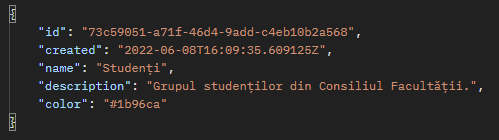
\includegraphics[width=115mm]{images/json_example.png}
    \caption{Exemplu de JSON folosit în aplicație}
\end{figure}

Nu în ultimul rând, pentru a menține \enquote{state-ul} în întregimea aplicației, am folosit librăria Redux. Aceasta este utilizată pentru a accesa și a modifica variabile necesare pe tot parcursul folosirii aplicației, precum starea autentificat / neautentificat sau datele utilizatorului (id, nume, prenume, etc.). Asemănător cu Chakra UI, pentru funcționarea librăriei a fost necesară punerea componentei principale întru-un provider customizabil, unde sunt declarate toate operațiile. 

\subsection{Structura aplicației server}

Aplicația server este realizată în limbajul Python, fiind folosit framework-ul Django, alături de librăria Django REST Framework ce permite utilizarea conceptelor de REST API în aplicație. Aplicația de backend este structurată de următoarele elemente importante pentru a funcționa eficient:

\begin{itemize}
    \item \enquote{Model}: definește reprezentarea schematică și structura unui obiect din baza de date, alături de legăturile pe care acesta le are cu alte obiecte.
    \item \enquote{Url}: reprezintă rutele unde se pot face cereri HTTP și face legătura dintre funcțiile aplicației și exterior.
    \item \enquote{View}: conține funcțiile apelate de către Url atunci când este accesată o rută și întoarce un răspuns HTTP.
    \item \enquote{Serializer}: transformă un model definit în Python în format JSON pentru a putea fi transmis mai departe de către View.
\end{itemize}

Framework-ul Django funcționează, în mare, pe modelul MVC (\enquote{Model View Controller}) \cite{MVC_what_is} și are la bază o multitudine de funcționalități, în special pe partea de View-uri. Aici sunt definite metodele și tipurile acestora (get, post, delete, etc.) și se împart în două categorii:

\begin{itemize}
    \item Metode aparținând unui \enquote{View Set}. View Set-ul este o clasă ce grupează mai multe metode pentru definirea rapidă a operațiilor de tip CRUD (\enquote{Create, Read, Update, Delete}) pentru un singur model.
    \item Metode de sine stătătoare. Metode ce sunt definite în afara View Set-urilor și au nevoie de o adnotare care să permită framework-ului să înțeleagă ce fel de cerere este făcută prin acea metodă, ca de exemplu: @GET, @PUT, @DELETE, etc..
\end{itemize}

De asemenea, pentru îndeplinirea unor funcționalități din interfața Voting App, a fost necesară trimiterea de email-uri. Pentru a realiza acest lucru eficient a fost folosit conceptul de multithreading. Astfel, atunci când era cerută trimiterea unui mail, aplicația de backend crea un nou fir de execuție pentru a o procesa, putând, astfel, gestiona în continuare alte cereri.

\subsection{Baza de date}

Pentru a salva datele procesate de către aplicația server, am folosit o bază de date MySQL. Legătura dintre MySQL și Django a fost realizată utilizând funcționalitatea integrată în framework. De asemenea, în baza de date au fost folosite și alte tabele în afară de cele pentru modelele definite precum:

\begin{itemize}
    \item \enquote{django\_rest\_passwordreset}, utilizat pentru a salva date necesare procesului de resetare a parolei de către utilizator.
    \item \enquote{django\_migrations}, folosit pentru a memora date despre migrațiile făcute în baza de date.
\end{itemize}

\begin{figure}[!h]
    \centering
    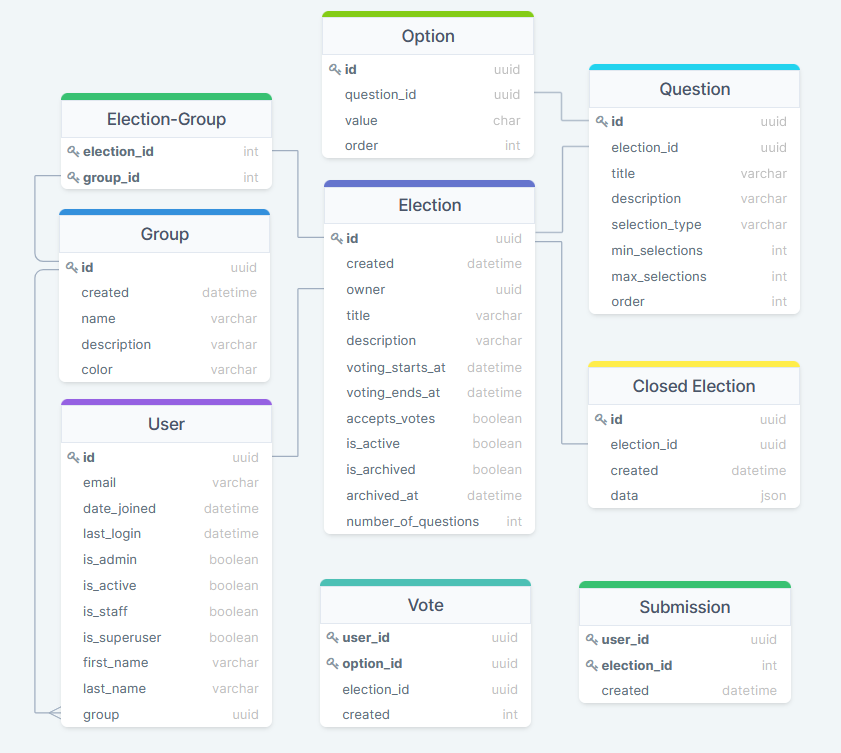
\includegraphics[width=135mm]{images/db_example.png}
    \caption{Diagrama structurii și relațiilor modelelor din baza de date}
\end{figure}
